% !TEX root=../master.tex
\chapter{GPS Denied Orbit Control}
\label{ch:orbit_control}
% - interesting because of the GPS denied aspect

Once the handoff vehicle has obtained a reasonable estimate of the relative transform between itself and the tracking UAV, it is equipped to insert itself into a similar orbit about the target.
Because there is no GPS-data available, the orbit control must only use estimates of the target's position and velocity relative to the vehicle.
Initially, the handoff UAV will use the relative pose information to compute the LOS between itself and the target according to Equation~\eqref{eq:target_rel_pos}, but by the time the target handoff is complete, it will need to orbit the target based entirely on visual data.

Another challenge of GPS-denied orbiting is that the vehicle cannot use global waypoints or orbit centers to loiter about the target, but must instead give heading rate or roll commands.
The implementation here assumes the ability to command roll directly, but the derivation for commanding heading rate would be similar.
This section describes the control used to compute appropriate roll commands from the target's relative position and velocity.
We also discuss how we orbit the target using only visual information after the handoff is complete.

\section{Orbit Control}

\subsection{Target relative state}
As previously noted, without GPS, the state of the target must be represented relative to the UAV. We will represent the state of the target as
\begin{equation}
    \x_\tg = \pmat[1.5]{\ptghv \\ \veltghv}\;,
\end{equation}
where the target position represents the line of sight vector frome the UAV to the target and the target velocity represents the motion of the target relative to the UAV.

In the context of the orbit control, it is more intuitive to think of the target as being stationary, with the handoff vehicle moving with some velocity relative to the target.
Accordingly, in the control derivation, we refer to the relative velocity as $\velhtg$, which is just the negative of the target's velocity relative to the UAV, according to
\begin{equation}
    \velhtg = -\veltghv\;.
\end{equation}

Because the target is in motion, a constant radius orbit about the target would take the form of a spiral in the world xy-frame.
Rather than attempting to follow a spiral trajectory in the world frame, we can simplify the problem by controlling the UAV to follow a constant radius orbit in the target relative frame.
The end result is analagous to controlling a constant orbit in the presence of wind.

In order to maintain a constant orbit in the relative frame, the UAV must maintain a $90^\degree$ angle between the relative velocity vector and the line of sight vector to the target.
This angle will be denoted by $\gamma$.
The angle between the x-axis of the vehicle and the line of sight vector to the target will be given by $\az$, which correpsonds with the azimuth of the gimbal.
Figure~\ref{fig:target_relative_vectors} gives a visual representation of these vectors and angles.
\begin{figure}[hbt]
    \centering
    \includegraphics[width=0.5\columnwidth]{figures/target_vel_vectors}
    \caption{Depiction of target relative position, velocity, and related angles.}
    \label{fig:target_relative_vectors}
\end{figure}

\subsection{Control implementation}

The goal of the orbit control is to cause the UAV to fly directly towards the target when it is very far away ($\gamma = 0$) then to gradually drive $\gamma$ to $\frac{\pi}{2}$ when the distance between the target and the UAV approaches the desired orbit radius.

The value of $\gamma$ is computed according to
\begin{equation}
    \gamma = \atantwo\left(\norm{\vel_{\HwrtTG}\cross\ptghv}, \hspace{1em}\vel_{\HwrtTG}\cdot\ptghv\right)\;.
\end{equation}
% While the dot product or cross product alone is sufficient to get the magnitude of the angle between the two vectors, using $\atantwo$ on the quotient of the cross and dot products allows us to determine the proper direction of the angle.

Using the equations for angular velocity in an orbit and the coordinated turn condition for fixed-wing aircraft, we can derive an expression for the desired roll command according to
\begin{align}
    \dot{\gamma} &= \frac{\norm{\vel_{\HwrtTG}}}{R} \\
    &= \frac{g}{\norm{\vel_{\HwrtTG}}}\tan\phi\\
    \label{eq:phi_ff}
    \phiff &= \atan\left(\frac{\norm{\vel_{\HwrtTG}}^2}{gR}\right)\;.
\end{align}

We use the expression in \eqref{eq:phi_ff} as the feed forward term to keep the UAV in a proper orbit.
We also add PD control on $\gamma$ to help the UAV converge onto the proper orbit.
The full roll control becomes
\begin{align}
  \phi_{c} &= \phiff+k_{p}e_{\gamma}+k_{d}\dot{e}_{\gamma}\\
  e_{\gamma} &= \gamma-\gamma_{d}\;.
\end{align}

We want the aircraft to converge to the desired orbit with the appropriate direction (clockwise or counter-clockwise) and radius as quickly as possible. Accordingly, the desired value for $\gamma$ should allow the UAV to fly directly toward or away from the target to quickly approach the desired radius, and then to smoothly transition to the tangential motion of an orbit in the proper direction. To accomplish this, we added an arctangent term to make a smooth transition between the desired range-dependent far-field and near-field behaviors. The expression for the desired $\gamma$ becomes
\begin{equation}
    \gamma_{d} = \lambda\left[\atan\left(-\beta\left(R-R_{d}\right)\right)+\frac{\pi}{2}\right]\;,
\end{equation}
where $\lambda$ represents the direction of the orbit ($+1$ for clockwise and $-1$ for counter-clockwise) and $\beta$ is a constant to control the rate at which $\gamma_d$ should transition from the perpendicular motion to the tangential motion as it approaches the proper orbit.
%% ST: Maybe add something here about choosing beta based on system constraints

\section{Vision-based Orbiting}
 Visual information provides a more reliable measurement of the target's relative position than the relative LOS that is initially used to orbit the target, but it also requires that the UAV maintain the target in the field of view and keep a consistent track in order to receive information.

\subsection{Target position estimation}
Initially the handoff UAV must rely on the information from the relative pose particle filter to estimate the target's position according to
\begin{equation} \label{eq:target_pos_rel}
    \ptghv = \p_{\TwrtH}^\hv + \Rot{\tv}{\hv}\Rot{\tb}{\tv}\p_{\TGwrtT}^\tb\;,
\end{equation}
where $\p_{\TwrtH}^\hv$ and $\Rot{\tv}{\hv}$ are estimates from the particle filter, $\Rot{\tb}{\tv}$ comes from the tracker's complimentary attitude filter, and $\p_{\TGwrtT}^\tb$ is measured by the tracker. Because the value of $\ptghv$ is the product of several estimated and measured values, each with their own noise and uncertainty, it will be relatively noisy. It does contain enough information to help the UAV navigate in the right direction and get the target into the field of view of the camera.
Once the handoff UAV is sufficiently confident that it has found the correct target, it can begin utilize visual information to orbit the target, becoming independent of measurements from the tracking UAV in preparation for tracking UAV's departure.

As long as the handoff UAV can maintain the target in the field of view and keep track of the target visually, the visual information provides a reliable measurment of the relative position of the target.
In order to estimate the target's position, the UAV must transform the line of sight into the proper frame with the proper scale. The handoff UAV's target tracking algorithm will produce the target's position in normalized image plane pixel coordinates of the handoff UAV's camera.

Let
\begin{equation}
    \pimgvec_{\TGwrtH} = \pmat{\pimgvar_x \\ \pimgvar_y \\ 1}
\end{equation}
represent the normalized image coordinates of the target received from the tracker. Normalized image coordinates are normalized by the focal length of the camera in pixels, so that they are independent of the camera intrinsics.
Converting $\pimgvec_{\TGwrtH}$ to a unit vector, we get
\begin{equation}
    \ptg[\check]^c = \frac{\pimgvec_{\TGwrtH}}{\norm{\pimgvec_{\TGwrtH}}}\;.
\end{equation}
We rotate the normalized LOS into the handoff vehicle 1 frame according to
\begin{equation}
    \ptghv[\check] = \Rot{\hb}{\hv}\Rot{g}{\hb}\Rot{c}{g}\ptg[\check]^c\;,
\end{equation}
where $\Rot{c}{g}$ is a fixed rotation given by
\begin{equation}
    \Rot{c}{g} = \pmat{
      0 & 0 & 1 \\ 1 & 0 & 0 \\ 0 & 1 & 0
      }\;,
\end{equation}
$\Rot{g}{\hb}$ can be constructed from the gimbal azimuth ($\az$) and elevation ($\el$) as
\begin{equation}
    \Rot{g}{\hb} = \pmat{\cos\el\cos\az & -\sin\az & \sin\el\cos\az \\
                         \cos\el\sin\az &  \cos\az & \sin\el\sin\az \\
                         -\sin\el       &  0       & \cos\el}\;,
\end{equation}
and
\begin{equation}
  \Rot{\hb}{\hv} = \Rot{\theta}{}\Rot{\phi}{}\;,
\end{equation}
with $\Rot{\theta}{}$ and $\Rot{\phi}{}$ defined by equations \eqref{eq:R_theta} and \eqref{eq:R_phi}.

Using a flat-earth assumption, we can recover the appropriate scale of the LOS using the altitude of the vehicle, according to
\begin{align}
    k &= \frac{h}{\e_3^\transpose\ptghv[\check]} \\
    \label{eq:ptg_vis_scaled}
    \ptghv &= k\hspace{0.1em}\ptghv[\check]\;.
\end{align}
This visually-derived estimate of the target's position can then be used to improve or replace the estimate given by Equation~\eqref{eq:target_pos_rel}.

\subsection{Target velocity estimation}
A good estimate of the target's position allows the UAV to track and orbit the target more effectively, but it is possible that the UAV will momentarily lose track of the target. Especially when the UAV is orbiting the target using only visual information, it is important for the UAV to have an estimate of the target's motion so that the UAV can maximize the likelihood that it will continue moving the right direction and keep the target in the field of view of the camera.

There are three main ways that we can estimate the target's velocity. We can use velocity information from the visual tracker, we can extract velocity information by differencing LOS estimates, and we can use the orbit control to infer information about the target's velocity.

\paragraph{Visual velocity}
The first method for estimating the target's velocity is to use information from the visual tracker. The R-RANSAC target tracking algorithm uses a Kalman filter to estimate and propagate the motion of the target based on successive visual measurements. The algorithm provides the estimated velocity of the target from the Kalman filter given in the normalized image plane, which we will represent as
\begin{equation}
    \vimgvec_{\TGwrtH} = \pmat{\vimgvar_x \\ \vimgvar_y \\ 0}\;.
\end{equation}
Note that the $z$-component is zero because the velocity is measured in the image plane and has no depth along the camera $z$-axis.

In order to keep the proper proportions between the velocity and position vectors, the velocity is scaled and rotated by the same amounts as the LOS, according to
\begin{equation} \label{eq:vtg_vis_hv}
    \veltghv[\bar] = k \left( \Rot{\hb}{\hv}\Rot{g}{\hb}\Rot{c}{g} \frac{\vimgvec_{\TGwrtH}}{\norm{\pimgvec_{\TGwrtH}}}\right)\;,
\end{equation}
where $k$ is the same scaling value used Equation~\eqref{eq:ptg_vis_scaled}.

Because the velocity measured by R-RANSAC is a projection onto the image plane, there are an infinite number of vectors that would create the same projection. The velocity computed in Equation~\eqref{eq:vtg_vis_hv} is simply the solution that is parallel to the image plane. If we instead assume that the velocity is parallel to a flat ground plane, we can get a more accurate estimate of the velocity by unprojecting $\veltghv[\bar]$ to find the vector that is parallel to the ground plane, but which still projects to the same vector in the image plane.


\begin{figure}[hbt]
  \centering
  \includegraphics[width=0.6\columnwidth]{figures/target_velocity}
  \caption{Depiction of vectors used for computing the target's velocity using information from the visual tracker.}
  \label{fig:camera_vel_vectors}
\end{figure}

Let $\m$ represent the vector from the camera origin to the velocity vector, as shown in Figure~\ref{fig:camera_vel_vectors}, given by
\begin{equation}
    \m = \ptghv+\veltghv[\bar]\;.
\end{equation}
All valid velocities will lie along $\m$ such that
\begin{equation} \label{eq:vtg_vis_projections}
    \veltghv = \lambda \m - \ptghv\;,
\end{equation}
but we want the velocity vector that both satisfies Equation~\eqref{eq:vtg_vis_projections} and has zero $z$-component.
Accordingly, we can solve for $\lambda$ according to
\begin{align}
    \pmat{v_x \\ v_y \\ 0} &= \lambda \m - \ptghv \\
    \lambda &= \frac{\e_3^\transpose \ptghv}{\e_3^\transpose \m}\;,
\end{align}
allowing us to compute the most accurate visual measurement of the velocity as
\begin{align} \label{eq:vtg_vis_measurement}
    \veltghv[\tilde] &= \lambda \m - \ptghv \\
      &= \left(\frac{\e_3^\transpose \ptghv}{\e_3^\transpose \m} \right)\m - \ptghv\;.
\end{align}


\paragraph{Line-of-sight differencing}
The second method of estimating the target's velocity is to use the derivative of the target's relative position. The time derivative of the target's position is given by
\begin{equation}
    \ptghv[\dot] = -\skewmat{\angvel_{\HVwrtI}}\ptghv + \vel_{\TGwrtI}^\hv - \vel_{\HwrtI}^\hv\;.
\end{equation}
We can estimate the time derivative according to
\begin{equation} \label{eq:vtg_delta_pos}
    \frac{\Delta\ptghv}{\Delta t} \approx -\skewmat{\angvel_{\HVwrtI}}\ptghv + \vel_{\TGwrtI}^\hv - \vel_{\HwrtI}^\hv\;,
\end{equation}
and use this to extract information about $\vel_{\TGwrtI}^\hv$.

\paragraph{Orbit control output}
The third method for obtaining an estimate of the target's velocity is to use the output of the orbit controller. The orbit control is made up of a feed-forward term and an adaptive term. The feed-forward term includes the current estimate of the target's velocity, but it will initally be in accurate because we don't know how the target is moving. The adaptive term will make up the difference, allowing the combined control output to effectively orbit a moving target. Assuming that the roll command is accounting for the motion of the target correctly, we can use the roll command to extract information about how the target is moving.

The ideal roll command needed to maintain a constant radius orbit about a the target is expressed as
\begin{equation}
    \phi = \atan\left(\frac{\norm{\vel_{\HwrtTG}}^2}{gR}\right)\;.
\end{equation}
Accordingly, we can extract the magnitude of the relative velocity from the roll according to
\begin{equation} \label{eq:vrel_phi}
    \norm{\vel_{\HwrtTG}}^2 = gR\tan(\phi)\;.
\end{equation}
Expanding the norm, we get
\begin{align} \label{eq:vrel_norm}
  \norm{\vel_{\HwrtTG}}^2 &= (\vel_{\HwrtI} - \vel_{\TGwrtI})^\transpose (\vel_{\HwrtI} - \vel_{\TGwrtI}) \\
     &= \vel_{\HwrtI}^\transpose\vel_{\HwrtI}
        - 2\vel_{\HwrtI}^\transpose\vel_{\TGwrtI}
        + \vel_{\TGwrtI}^\transpose\vel_{\TGwrtI} \;.
\end{align}
Because this value is a scalar, we cannot directly reconstruct the target velocity, but instead must estimate it over time.

Assuming that the target motion is planar, \eqref{eq:vrel_norm} can be expressed in terms of the magnitude and direction of the
target velocity according to
\begin{align} \label{eq:target_vrel_theta}
    \norm{\vel_{\HwrtTG}}^2 &= \norm{\vel_{\HwrtI}}^2
       - 2\norm{\vel_{\HwrtI}}\norm{\vel_{\TGwrtI}}\cos\theta
       +\norm{\vel_{\TGwrtI}}^2 \nonumber\\
       &= v_a^2 - 2v_a V_{\tg} \cos\theta + V_{\tg}^2\;,
\end{align}
where $v_a$ is the airspeed of the handoff vehicle and $V_{\tg}$ is the magnitude of the target.
Solving Equation~\eqref{eq:target_vrel_theta} for $V_{\tg}$ and $\theta$ will provide a set of valid solutions, but when considered over time, there is a solution that best satisfies all the constraints.

Rather than solving for an analytical closed-form solution, we pose the target velocity estimation as an optimization problem. This allows us to incorporate each of the three sources of information and to weight them according to their reliability and usefulness. We also decompose the target velocity estimate into the magnitude, $\hat{V}$, and the relative heading, $\hat{\theta}$. Splitting up the velocity in this way allows us greater control over how we tune the performance of the optimization.

Let the cost function, $J(\hat{V}_{k},\hat{\theta})$, be defined by
\begin{equation}
    J_k(\hat{V}_{k},\hat{\theta}_k) = \sum\limits_{i=0}^{n-1} \gamma^i \left(w_v e_{v_{k-i}}^2 + w_p \norm{\e_{p_{k-i}}}^2 + w_\phi e_{\phi_{k-i}}^2\right) \;,
\end{equation}
where $e_{v}$, $e_{p}$, and $e_{\phi}$ represent the components of the cost derived from the visual information, the difference in position estimates, and the roll command respectively, each with their own weight, $w$. We also apply a temporal discount factor, $\gamma$, that allows us to place more weight on more recent measurements.

Let the visual error be defined as
\begin{align}
    e_{v_{k}}^2 &= e_{\norm{v}_k}^2 + e_{\theta_k}^2 \\
        &= \left( \hat{V}_k - \norm{\veltghv[\tilde]} \right)^2 + \left( \hat{\theta}_k - \atantwo(\tilde{V}_y, \tilde{V}_x) \right)^2\;,
\end{align}
where $\veltghv[\tilde]$ is the visual measurement of the velocity from Equation~\eqref{eq:vtg_vis_hv}. Because we directly measure the target's velocity visually, we can also break the error into the magnitude and angle components to simplify the gradients and allow for greater control over the individual parameters.

The gradients of $e_{v_{k}}^2$ with respect to $\hat{V}_k$ and $\hat{\theta}_k$ are given by
\begin{equation}
    \pardd[e_{v_{k}}^2]{\hat{V}_k} = 2e_{\norm{v}_k}
\end{equation}
and
\begin{equation}
    \pardd[e_{v_{k}}^2]{\hat{\theta}_k} = 2e_{\theta_k}\;.
\end{equation}

We define the error from the difference in position estimates, $e_{p_{k}}$, using Equation~\eqref{eq:vtg_delta_pos} as
\begin{equation}
    \e_{p_{k}} = \left(-\skewmat{\angvel_{k}}\p_{k-1} + \hat{V}_k\pmat{\cos\hat{\theta}_k \\ \sin\hat{\theta}_k \\ 0} - \vel_{h_k} \right) - \frac{\p_k - \p_{k-1}}{\Delta t}\;,
\end{equation}
with gradients
\begin{equation}
    \pardd[\norm{\e_{p_{k}}}^2]{\hat{V}_k} = 2\e_{p_{k}}^\transpose \pmat{\cos\hat{\theta}_k \\ \sin\hat{\theta}_k \\ 0}
\end{equation}
and
\begin{equation}
    \pardd[\norm{\e_{p_{k}}}^2]{\hat{\theta}_k} = 2\hat{V}_k\e_{p_{k}}^\transpose \pmat{-\sin\hat{\theta}_k \\ \cos\hat{\theta}_k \\ 0}\;.
\end{equation}

The error derived from the roll command is obtained by combining \eqref{eq:vrel_phi} and \eqref{eq:target_vrel_theta}, according to
\begin{equation}
    e_{\phi_{k}} = \left(v_a^2 - 2v_a \hat{V}_{k} \cos(\hat{\theta}_k) + \hat{V}_{k}^2\right) - gR\tan(\phi) \;.
\end{equation}
The gradients with respect to $e_{\phi_{k}}^2$ are given by
\begin{equation}
    \pardd[e_{\phi_{k}}^2]{\hat{V}_{k}} = 4e_{\phi_{k}}\left(\hat{V}_{k} - v_a\cos\hat{\theta}_k \right)
\end{equation}
and
\begin{equation}
    \pardd[e_{\phi_{k}}^2]{\hat{\theta}_{k}} = 4e_{\phi_{k}}\left(v_a\hat{V}_{k}\sin\hat{\theta}_k \right)\;.
\end{equation}

The full gradients, then, are given by
\begin{align}
  \pardd[J_k(\hat{V}_{k},\hat{\theta}_{k})]{\hat{V}_{k}} &= \sum\limits_{i=0}^{n-1} \gamma^i \Bigg[
        w_v\pardd[e_{v_{k-i}}^2]{\hat{V}_{k-i}} + w_p\pardd[\norm{\e_{p_{k-i}}}^2]{\hat{V}_{k-i}} + w_\phi\pardd[e_{\phi_{k-i}}^2]{\hat{V}_{k-i}} \Bigg]
\end{align}
        % \\
        % &= \sum\limits_{i=0}^{n-1} \gamma^i \Bigg[
        %    2e_{\norm{v}_{k-i}}
        %    + 2\e_{p_{k-i}}^\transpose \pmat{\cos\hat{\theta}_{k-i} \\ \sin\hat{\theta}_{k-i} \\ 0} \nonumber\\
        %    &\hspace{4em}+ 4e_{\phi_{k-i}}\left(\hat{V}_{k-i} - v_a\cos\hat{\theta}_{k-i} \right)\Bigg]
% \end{align}
and
\begin{align}
  \pardd[J_k(\hat{V}_{k},\hat{\theta}_{k})]{\hat{\theta}_{k}} &= \sum\limits_{i=0}^{n-1} \gamma^i \Bigg[
        w_v\pardd[e_{v_{k-i}}^2]{\hat{\theta}_{k-i}} + w_p\pardd[\norm{\e_{p_{k-i}}}^2]{\hat{\theta}_{k-i}} + w_\phi\pardd[e_{\phi_{k-i}}^2]{\hat{\theta}_{k-i}} \Bigg]
\end{align}
        % \\
        % &= \sum\limits_{i=0}^{n-1} \gamma^i \Bigg[
        %    w_v 2e_{\theta_{k-i}} \nonumber\\
        %    &\hspace{4.5em}+ w_p 2\hat{V}_{k-i}\e_{p_{k-i}}^\transpose \pmat{-\sin\hat{\theta}_{k-i} \\ \cos\hat{\theta}_{k-i} \\ 0} \nonumber\\
        %    &\hspace{5.5em}+ w_\phi 4e_{\phi_{k-i}}\left(v_a\hat{V}_{k-i}\sin\hat{\theta}_{k-i} \right)\Bigg]\;.
% \end{align}

Note that becuase the cost function is composed of errors from the past $n$ timesteps, the gradients include past estimates of the velocity. In order to optimize the current estimates based on multiple time steps, we want the gradient to be a function of only the current estimates, $\hat{V}_{k}$ and $\hat{\theta}_k$.
To express past estimates in terms of the current magnitude and angle, we can make the substitution
\begin{equation}
    \hat{\theta}_{k-i} = \hat{\theta}_k + \Delta \theta_i \;,
\end{equation}
where
\begin{equation}
    \Delta \theta_i = \Delta t\sum\limits_{j=1}^i \omega_{k-j} \;,
\end{equation}
and $\omega$ is the angular velocity about the $z$-axis. The target speed does not have this same issue because we assume that the speed is nearly constant through time, so
\begin{equation}
    \hat{V}_{k-i} = \hat{V}_k\;.
\end{equation}

At each optimization iteration, the estimated values, $\hat{V}$ and $\hat{\theta}$ are updated according to
\begin{align}
    \hat{V}^+_{k} = \hat{V}_{k} - l_V \pardd[J_k(\hat{V}_{{k}},\hat{\theta}_{k})]{\hat{V}_{{k}}}\;, \\
    \hat{\theta}^+_{k} = \hat{\theta}_{k} - l_\theta \pardd[J_k(\hat{V}_{{k}},\hat{\theta}_{k})]{\hat{\theta}_{k}}\;,
\end{align}
where $l_V$ and $l_\theta$ are tunable learning rates for the velocity magnitude and angle respectively.
At each time step, we perform multiple optimization iterations, updating the estimates and gradients with each iteration.


\section{Results}
We implemented this control scheme in the full handoff simulation with noise on all sensors and using estimated values for the target LOS as the input to the control. The orbit control quickly converged onto the desired orbit and allowed the handoff vehicle to keep the target in the field of view to begin tracking and perform the handoff. Initially the handoff UAV must rely on the outputs of the relative- and self-pose filters to estimate the target's position and despite the noise in both estimators, the orbit control accomplishes the desired task of effectively following a moving target without GPS. Figures~\ref{fig:orbit_position}~and~\ref{fig:orbit_rel_position} show the position of the target and handoff vehicle in the $xy$-plane and Figure~\ref{fig:orbit_error} shows the orbit radius error over time.

\begin{figure}[hbt]
  \centering
  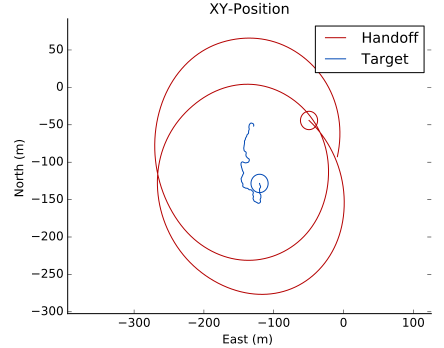
\includegraphics[width=0.7\columnwidth]{figures/orbit_position}
  \caption{Plot of the handoff UAV orbiting the target.}
  \label{fig:orbit_position}
\end{figure}

\begin{figure}[hbt]
  \centering
  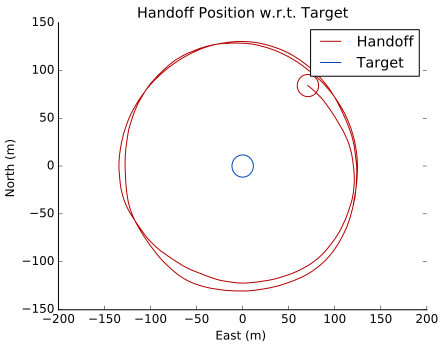
\includegraphics[width=0.7\columnwidth]{figures/orbit_rel_position}
  \caption{Plot of the handoff orbit relative to the target.}
  \label{fig:orbit_rel_position}
\end{figure}

\begin{figure}[hbt]
  \centering
  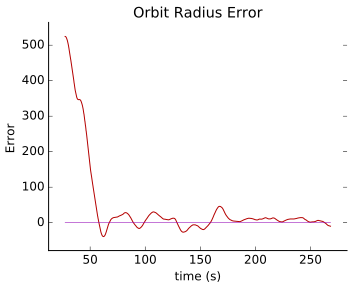
\includegraphics[width=0.7\columnwidth]{figures/orbit_error}
  \caption{Handoff orbit radius error over time.}
  \label{fig:orbit_error}
\end{figure}
